\section{\textit{Fog computing}}

Иако се \textit{edge} и \textit{fog computing} често спомињу у истом контексту и неретко користе као синоними, постоји значајна разлика између ова два појма. \textit{Fog computing} представља унапређење \textit{edge computing}-а проширујући његове могућности обраде и складиштења података увођењем \textit{fog} чворова који се налазе између \textit{edge} и \textit{cloud} система. У суштини, он је екстензија \textit{cloud}-а с тиме да је много ближи уређајима \textit{edge} система \ref{fig:fog_arch}, што великим делом очувава све погодности \textit{edge computing}-а као што су брза мрежна комуникација, мала латенција и безбедност, а опет омогућава обраде података које захтевају много веће рачунарске ресурсе. Овако \textit{edge} систем још увек може самостално да обрађује најкритичније податке по безбедност и брзину рада апликације, а да остатак посла делегира \textit{fog} чворовима. Још једна од погодности је могућност много већег географског распростирања једног система користећи горе поменуте \textit{fog} чворове. 

\begin{figure}[H]
    \centering
    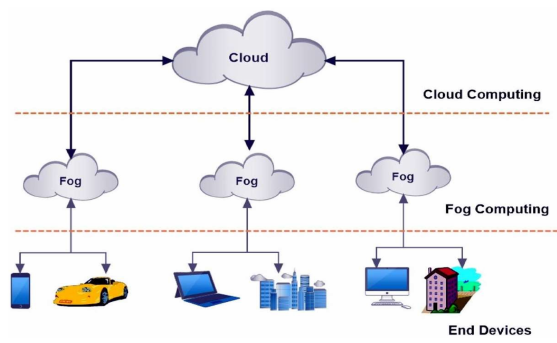
\includegraphics[width=1\textwidth]{images/fog_arch.png}
    \caption{\textit{Fog} је попут \textit{cloud}-а који је много ближи крајњим уређајима}
    \label{fig:fog_arch}
\end{figure}

\pagebreak
\subsection{Архитектура}

Архитектура \textit{fog computing}-a састоји се из шест слојева \ref{fig:fog_layers}:

\begin{figure}[H]
    \centering
    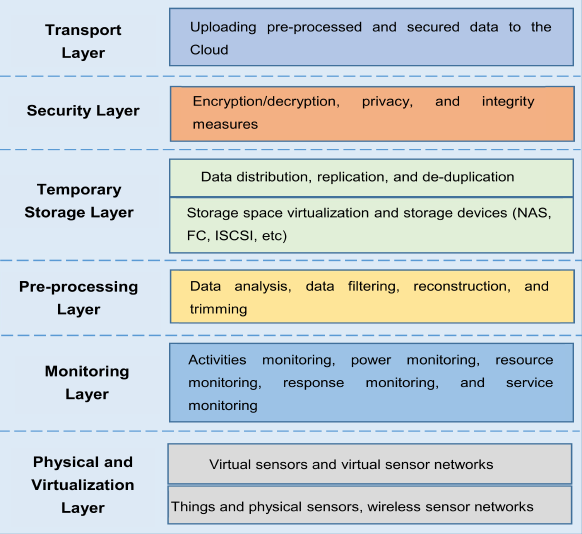
\includegraphics[width=1\textwidth]{images/fog_layers.png}
    \caption{Слојевита архитектура \textit{fog computing}-a}
    \label{fig:fog_layers}
\end{figure}

Физички и виртуелизациони слој укључује различите типове чворова попут физичких, виртуелних чворова или виртуелних сензорских мрежа. Различити чворови географски су дистрибуирани да би прикупили информације из њихове околине и послали их вишим слојевима уз помоћ \textit{gateway}-a на даље филтрирање и процесирање.

Слој за надзор прати искоришћење ресурса, доступност сензора и \textit{fog} чворова, као и осталих елемената мреже. Сви задаци које обављају чворови се прате у овом слоју, пратећи који чвор обавља који задатак, у које време, и шта ће му бити потребно у наредном кораку. Прате се перформансе и статус свих апликација и услуга које су имплементиране унутар система. Додатно, прати се и потрошња енергије \textit{fog} чворова.

У пре-процесном слоју сакупљени подаци се анализирају, врши се филтрирање и редуковање података како би се извукле значајне информације. Претпроцесирани подаци се затим складиште у слоју за привремено складиштење. Када се подаци пренесу на \textit{cloud}, више им није потребно локално складиштење и могу бити уклоњени са привремених складишних медија.

Безбедносни слој врши шифровање и дешифровање података, а често и примењује мере заштите њиховог интегритета, како их потенцијални нападачи не би могли неприметно прочитати или изменити приликом њиховог транспорта на \textit{cloud}.

На самом крају, у транспортном слоју, претпроцесирани подаци се транспортују на \textit{cloud} како би се издвојили и креирали додатни корисни сервиси. Ради ефикасне употребе енергије и очувања безбедности података, само део сакупљених података се транспортујe на \textit{cloud}. 

\subsection{Могуће примене}

Тренутна централизована архитектура \textit{cloud computing}-a суочава се са озбиљним изазовима за \textit{IoT} апликације. На пример, не може да подржи временски осетлљиве \textit{IoT} апликације, као што су \textit{video streaming, gaming} и \textit{augmented reality}. Такође, недостаје свест о локацији процеса, јер је у питању централизовани модел. \textit{Fog computing} може да реши ове изазове. \textit{Fog computing} делује као мост између \textit{IoT} уређаја и великих \textit{cloud} рачунарских и складишних услуга. Он пружа високо виртуализовани модел рачунања, складиштења и мрежних ресурса између крајњих уређаја и класичних \textit{cloud} сервера.

\subsubsection{Аутономна возила}

Постоје многе корисне функционалности, које зависе од \textit{fog}-a и интернет конекције, које могу бити додате аутомобилима као што су "\textit{hands free}" режим вожње или функција самопаркирања која више не би захтевала возача за воланом како би се аутомобил паркирао.
У следећих неколико година се очекује да ће сви нови аутомобили имати могућност комуникације са блиским аутомобилима и интернетом. \textit{Fog computing} ће бити најефикасније решење за сва возила повезана са интернетом, јер омогућава комуникацију у реалном времену. Такође, омогућиће аутомобилима, приступним тачкама и семафорима да комуницирају једни са другима како би обезбедили добру услугу корисницима.
Уз коришћење \textit{fog}-a уместо \textit{cloud}-a, судари и другe несреће могле би се свести на минимум.

\subsubsection{Паметне куће}

\textit{IoT} има многo повезаних сензора и уређаја унутар домаћинстава. Међутим, ови уређаји долазе од различитих произвођача и користе различите платформе, што отежава њихово међусобно повезивање. Такође, неки задаци захтевају велику количину рачунарских ресурса и простора за складиштење података. \textit{Fog computing} решава многе од ових проблема, интегрише све различите платформе и омогућава паметним кућним апликацијама приступ флексибилним ресурсима. \textit{Fog computing} такође пружа много предности за апликације за обезбеђивање домаћинстава.